\documentclass{amia}
\usepackage{graphicx}
\usepackage{pgfplots}
\usepackage{minted}
\usepackage{algorithmicx}
\usepackage{algorithm}
\usepackage{algpseudocode}
\usepackage{pgfplotstable}
\usepackage{booktabs} 
\usepackage{longtable}

\begin{document}

\title{High Throughput Phenotyping -- Architectural Review}

\author{ 
     ....
}

\institutes{
    $^1$ Mayo Clinic, Rochester, MN
}

\maketitle

\section*{Abstract}

\textit{Effectively executing phenotyping algorithms on large populations of patients requires a multifaceted engineering approach. First, the standards-based algorithm representation must be transformed into a machine executable artifact. Next, the computation engine must allow for horizontal as well as vertical scalability. Finally, the resultant analytic information must be collated such that a useful response can ultimately returned. The High Throughput Phenotyping (HTP) project utilizes the The Quality Data Model (QDM) format for algorithm specification, allowing for standardization and interoperability. The QDM model is then converted to a JBoss{\textsuperscript{\textregistered}} Drools representation, which can then be executed in a clustered environment. Deployment in a clustered environment allows for horizontal scalability.}

\section*{Introduction}
The Strategic Health IT Advanced Research Projects (SHARP) Program established a platform for analyzing normalized clinical patient data\cite{pathak2013normalization,rea2012building}. The SHARP project focuses on many facets of patient data analytics, such as data normalization (in terms of semantics as well as structure), as well as a standards based focus. For this work, we focus on an important aspect of this technological stack, the computation engine. 

\section*{Methods}
We base our architectural evaluation on a concrete use-case, the execution of a National Quality Forum (NQF) algortithm, specifically, \textit{Aspirin Prescribed at Discharge - (NQF: 0142)}, which aims to identify Acute myocardial infarction (AMI) patients who are prescribed aspirin at hospital discharge. For our analysis, we make two assumptions, that the given algorithm is available in Quality Data Model (QDM) XML format, and that an arbitrary set of patient data is available.

In order to evaluate a candidate architecture, we first present a series of architectural principals that outline the critical high-level functional and non-functional requirements of the system. These principals guide design decisions and technology choices, and must hold for the candidate architecture to be viable. Next, we examine the individual components of the system, along with either interconnections, along the an examination of general architectural style choices. To reinforce these ideas, the \textit{Aspirin Prescribed at Discharge} algorithm will be shown at various stages of transformation and ultimately computation. Finally, to test our viability hypothesis, we quantitatively measure system performance in terms of algorithm computation time, and execution ``correctness,'' or verification of the computation results.

\subsection*{Architecture}
//todo -- Describe high level architecture -- high level description of figure~\ref{htp-drools-arch} -- etc.

\textbf{Architectural Principals.}
In order to better understand the intent and function of the system, we have identified several guiding concepts, or architectural principles\cite{garlan1993introduction}.

\textbf{Principle 1: Standards Based}\\
\textbf{Statement:} Communications, interfaces, and data exchanges should be based on industry standards and specifications wherever possible.\\
\textbf{Rational:} Standards based design allows for effective componitization of the system, as component interfaces and data contracts can be linked to published specifications. This allows for low-coupling of functional modules, as well as improved separation of concerns. A standards based approach to design also allows for implementation and information \textit{hiding}\cite{sullivan2001structure}, which allows greater opportunities for substituting component implementations based on context and use-case.\\
\textbf{Implications:} There are several areas where standards will be used. First, and standard \textit{algorithm input format} is needed. This will allow interoperability and a common, shared grammar for communicating phenotyping algorithm intent. Second, as structured vocabularies play a major role in the algorithm logic, a standard terminology service interfaces is required. Finally, standard protocols are needed to integrate these components and to interact with the system.

\textbf{Principle 2: Testability}\\
\textbf{Statement:} System results should be verifiable, repeatable, and comparable to standard, curated data sets.\\
\textbf{Rational:} Phenotyping occurs in many domains, and although there are efforts to automate the process\cite{chung2008automated,kyzar2011towards}, in many instances it remains a manual, human-driven process\cite{tao2013phenotyping}. This presents a system testing problem, as it may be difficult to determine acceptable system outputs. It is important, therefore, that a subject matter expert curated test data set be available, and that the test infrastructure incorporate this such that testing is automated and repeatable.\\
\textbf{Implications:} Testing infrastructure will need to accommodate the automation of these test data sets. This also will require reporting processes available to clearly demonstrate test results.

\textbf{Principle 3: Adaptability}\\
\textbf{Statement:} The system will allow for patient phenotyping an a wide range of contexts and environments.\\
\textbf{Rational:} When accessing Electronic Health Record (EHR) data across institutional boundaries, significant interoperability challenges arise\cite{chute2011sharpn}. As such, it is important that the system not be coupled to a particular data set or execution environment.\\
\textbf{Implications:} Input data types need to be as general as possible, allowing for \textit{late binding} of the source data format to the phenotyping data execution format. The main requirement of this style is that adjacent components agree upon data exchange interfaces. 

\begin{figure}
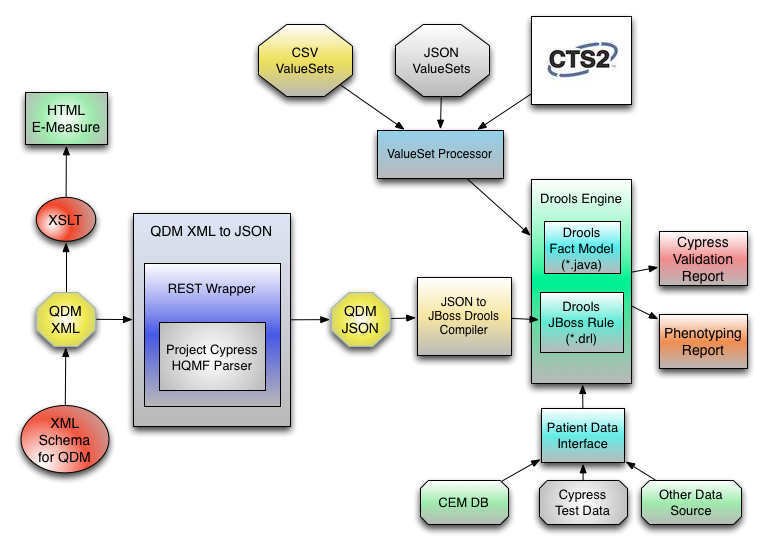
\includegraphics[width=\textwidth]{htp-drools-arch}
\caption{Phenotyping Architecture} 
\label{fig:overall_arch}
\end{figure}

\subsection*{Style}
The architectual style of the HTP execution engine is largely \textit{pipe and filter} based. In this style, input data is transformed via several discrete components in a streaming fashion, creating an information flow through the system which ultimately leads to the desired output\cite{garlan1993introduction}. One of the main benefits of this style is the strong separation of concerns of the components. Components need not know implementation details of each other -- and furthermore, need not even be aware of any other component, save those immediately adjacent to them in the pipeline. This implementation is possible via our Architectural Principle 1 - \textit{Standards Based} design, as components will have explicit and standardized contracts.

\subsection*{System Components}
\textbf{QDM XML to JSON Transformer.}
The QDM XML to JSON transformation component parses the QDM XML representation and transforms it into easily parsable JSON. This functionality is exposed via a REST service wrapping the Project Cypress health-data-standards\footnote{https://github.com/projectcypress/health-data-standards} project. This component is a Ruby\footnote{https://www.ruby-lang.org/en/} based component, and represents the only non Java Virtual Machine (JVM) component of the architecture.

\textbf{JSON to JBoss Drools Compiler}
The QDM JSON representation is programatically transformed into executable JBoss Drools rules via a compilation process. The result of this transformation is a single Drools Rules file that can be executed by the Drools Engine, or other JBoss Drools environment. The compilation component is based on the Groovy\footnote{http://groovy.codehaus.org/} language, as Groovy provides templating and string interpolation functionality that is difficult to replicate in Java.

\textbf{Drools Execution Engine}
Using the JBoss Drools engine, the generated Drools Rules can be executed given an input patient set. The result of this execution will be the patent set result mapped to the given populations (such as NUMER, DENOM, etc). A thin interface facade was created over the JBoss Drools version 5.6.0.Final library, hiding the implementation details of the engine. There are, in fact, no Drools-related APIs exposed to the client -- so the Drools-based implementation is decoupled from the user-facing APIs. This was done to allow flexibility in implementation, especially looking forward to moving to a Drools 6.x based implementation.\\
The interface \texttt{edu.mayo.qdm.executor.Executor} is the main entry-point for user interaction. It is through this interface that the engine can be started, and patient data processed. This interface accepts an \texttt{Iterable} collection of patients as input, allowing for user-specific implementations of patient \texttt{Iterators}. Because of this, users may hide implementation details behind the \texttt{Iterator} interface, allowing for a wide variety of data extraction techniques. For example, a patient \texttt{Iterator} may be implemented by a database result set, with custom cursors and pagination tailored to the specific database and environment. In fact, the \texttt{Iterator} need not be implemented based on persisted data at all -- but rather accept outputs from a streaming API or another analytics package.

\textbf{ValueSet Processor}
QDM Data Elements semantically defined their intended criteria by using \textit{Value Sets}, or enumerated sets of coded concepts from standard vocabularies. For instance,\\

\texttt{"Diagnosis, Active: Acute Pharyngitis" using "Acute Pharyngitis Grouping Value Set (2.16.840.1.113883.3.464.1003.102.12.1011)"}\\

In this example, in order for a QDM Data Element to be satisfied, a patient record must contain a Diagnosis entry coded with a Concept contained in the Value Set identified by the HL7 OID \texttt{2.16.840.1.113883.3.464.1003.102.12.1011}. These OIDs give the \textit{Value Set} global identity and enable interoperability accross systems\cite{steindel2010oids}.

For the purposes of algorithm execution, a mechanism for resolving the enumerated Concepts of a \textit{Value Set} is needed. Practically, it is usually advantageous to defer explicit resolution in favor of a \textit{exists}-type functionality. For example:

\begin{algorithm}
\begin{algorithmic}[1]
\Procedure{exists\_valueset}{oid, codedentry}
  \State $C \gets \{c | c \in resolve(oid)\}$
  \State \Return{ $coded\_entry \in C$ }
\EndProcedure
\end{algorithmic}
\end{algorithm}

Furthermore, it is necessary to find the subset of coded entries that align semantically with a defined  \textit{Value Set}. Extending the above example, it may be necessary to identify all Diagnoses in a patient record that align with the \texttt{2.16.840.1.113883.3.464.1003.102.12.1011} Value Set in order to do further processing or filtering, such as temporal relations. This function, described below, comprises the second point of functionality for the ValueSet Processor.

\begin{algorithm}
\begin{algorithmic}[1]
\Procedure{find\_matches}{oid, coded\_elements}
  \State $C \gets \{c | c \in resolve(oid)\}$
  \State \Return{ $C \cap coded\_elements$ }
\EndProcedure
\end{algorithmic}
\end{algorithm}

\subsection*{Standards, Models, and Processing Algorithms}
\textbf{QDM/HQMF.}
The Quality Data Model (QDM)\cite{behilngquality}...

\textbf{CTS2.}
Common Terminology Services 2\cite{cts2} is on Object Management Group{\textsuperscript{\textregistered}} (OMG) terminology services specification. This standard defines a common data model and interface for interacting with a terminology service, including read/write access and various maintenance, content loading, and querying functionality. CTS2 is the recommended implementation of the \textit{ValueSet Processor}, and can be easily incorporated via the provided adapter.

\textbf{Map Reduce.}
Map Reduce is computational abstraction designed to allow for easier parallelization and distribution of large data sets for processing\cite{dean2008mapreduce}. The computation is a two-step process, consisting of a \textit{map} function followed by a \textit{reduce} function. The \textit{map} function, given in input, divides this input into smaller sub-problems which then are consolidated by the \textit{reduce} function. Consider the example in figure~\ref{fig:map_reduce_example}, where the average height for a given age is calculated. The \textit{map} function iterates over the data collection, emitting for each record the age and height. This is then consolidated by the \textit{reduce} function, which given each key (or, each \textit{age}), computes the average height for that age.

\begin{figure}[H]
\begin{verbatim}
  map(String file, List children):
    for each child in children:
    	emit(child.age, children.height);

  reduce(String age, Iterator heights):
    emit(age, average(heights))
\end{verbatim}
\caption{Map Reduce Algorithm Example} 
\label{fig:map_reduce_example}
\end{figure}

We can apply this concept in the context of patients and populations. In the \textit{map} function, a function is applied to classify each patient into the appropriate populations given a phenotyping algorithm. We then reduce each population (and its given set of patients) into some analytic result -- for instance, analyzing demographic characteristics or creating patient lists for studies and clinical trials. Figure~\ref{fig:map_reduce_htp} illustrates this algorithm:

\begin{figure}[H]
\begin{verbatim}
  map(String algorithm, List patients):
    // key: phenotyping algorithm
    // value: List of patients
    for each patient in patients:
        for each population in getPopulations(algorithm, patient):
            emit(population, patient);

  reduce(String population, Iterator patients):
    // key: a population
    // values: a list of patients
    emit(population, postprocess(result))
\end{verbatim}
\caption{High Level Map Reduce Algorithm} 
\label{fig:map_reduce_htp}
\end{figure}

Figure~\ref{fig:map_reduce_htp} illustrates the general flow of information through the phenotyping algorithm. The \textit{getPopulations} function encompass the actual algorithm execution logic -- in our case, the \textit{Drools Execution Engine} component. The \textit{postprocess} function in the \textit{reduce} portion is left to be implemented by the client, as this will be use-case dependent. The code base does include a basic demographics analytics post processor, but it is expected that clients will extend it to meet their needs, or substitute their own processing entirely.

\textbf{Clustering.}
We follow the Hadoop clustering registration model\cite{wang2009hadoop}. The main advantage of this approach is that the master node does not need a priori knowledge of the number or location of the worker nodes. Using this approach, the master node, will accept incoming registration requests from worker nodes. These worker registration requests will include network location of the sending worker, which the master node then stores.

\subsection*{Execution Scenario - \textit{Aspirin Prescribed at Discharge - (0142)}}
To examine the functional capabilities of the system against a concrete use-case, we propose a prototypical usage scenario involving the NQF 0142 \textit{Aspirin Prescribed at Discharge} algorithm. Figure~\ref{fig:0142_IPP_text} shows the Initial Patient Population (IPP) definition of this algorithm in human-readable text format.

\begin{figure}[H]
\begin{verbatim}
 Initial Patient Population =
    AND: "Diagnosis, Active: Hospital Measures - AMI 
        (ordinality: 'Hospital Measures - Principal')" starts during "Occurrence A
        of Encounter, Performed: Hospital Measures-Encounter Inpatient"
    AND: "Patient Characteristic Birthdate: birth date" >= 18 year(s) starts before
        start of "Occurrence A of Encounter, Performed: 
        Hospital Measures-Encounter Inpatient"
    AND: "Occurrence A of Encounter, Performed: Hospital Measures-Encounter
        Inpatient (length of stay <= 120 day(s))"
    AND: "Occurrence A of Encounter, Performed: Hospital Measures-Encounter
        Inpatient (discharge datetime)" during "Measurement Period"
\end{verbatim}
\caption{NQF 0142 Text Representation} 
\label{fig:0142_IPP_text}
\end{figure}

The first step in the processing of this algorithm is to transform the logic conveyed in this human-readable representation into a machine executable format. Figure \ref{fig:0142_IPP_XML} shows the XML representation of the same logic described in Figure \ref{fig:0142_IPP_text}. The XML representation is based on the HL7 V3 RIM\cite{..hl7 citation here}.

\begin{figure}[H]
\begin{minted}{xml}
**************************************************************   
Population Criteria Section: population 
**************************************************************
<observation classCode="OBS" moodCode="EVN" isCriterionInd="true">
   <id root="64D92822-FB51-4A2B-840F-24DFCC91E4EB"/>
   <code code="ASSERTION" codeSystem="2.16.840.1.113883.5.4"/>
   <value xsi:type="CD" code="IPP" codeSystem="2.16.840.1.113883.5.1063"
          codeSystemName="HL7 Observation Value"
          displayName="Initial Patient Population"/>
   <!--  top and/or --><sourceOf typeCode="PRCN">
      <conjunctionCode code="AND"/>
      <act classCode="ACT" moodCode="EVN" isCriterionInd="true">
      <!-- Diagnosis, Active pattern -->
         ...
      </act>
   </sourceOf>
   <sourceOf typeCode="PRCN">
      <conjunctionCode code="AND"/>
      <act classCode="ACT" moodCode="EVN" isCriterionInd="true">
      <!-- Patient Characteristic Birthdate pattern -->
         ...
      </act>
   </sourceOf>
   <sourceOf typeCode="PRCN">
      <conjunctionCode code="AND"/>
      <act classCode="ACT" moodCode="EVN" isCriterionInd="true">
      <!-- Encounter, Performed pattern -->
         ...
      </act>
   </sourceOf>
   <sourceOf typeCode="PRCN">
      <conjunctionCode code="AND"/>
      <act classCode="ACT" moodCode="EVN" isCriterionInd="true">
      <!-- Encounter, Performed pattern -->
         ...
      </act>
   </sourceOf>
</observation>
</entry>
\end{minted}    
\caption{NQF 0142 XML Representation} 
\label{fig:0142_IPP_XML}
\end{figure}

\textbf{QDM JSON.}
Transformation begins by converting the XML representation in figure~\ref{fig:0142_IPP_XML} into a JSON representation, shown in figure~\ref{fig:0142_IPP_JSON}. The JSON representation has some notable advantages over the XML representation. First, the JSON representation makes a clear distinction between algorithm \textit{flow} and algorithm \textit{data elements}. Figure~\ref{fig:0142_IPP_JSON} exemplifies this notion for the IPP population definition. As shown the IPP population is comprised of \textit{precondition} objects, joined together by a boolean operator specified by the \textit{conjunction\_code} attribute. Notice that a \textit{precondition} can either contain nested \textit{preconditions} or \texttt{reference} a concrete \textit{data elements} for further processing. The JSON representation also assigns a unique identifier to each precondition (in the form of an \texttt{id} attribute. These identifiers take the form of incremental integers, and apply to all preconditions, whether they \texttt{reference} a concrete \textit{data element} or group other preconditions.


\begin{figure}[H]
\begin{verbatim}
IPP": {
    "conjunction?": true,
    "type": "IPP",
    "title": "Initial Patient Population",
    "hqmf_id": "64D92822-FB51-4A2B-840F-24DFCC91E4EB",
    "preconditions": [
    {
        "id": 54,
        "preconditions": [
        {
            "id": 46,
            "reference": "DiagnosisActiveHospitalMeasures...46"
        },
        {
            "id": 48,
            "reference": "PatientCharacteristicBirthdate...48"
        },
        {
            "id": 50,
            "reference": "OccurrenceAHospitalMeasuresEncounterInpatient...50"
        },
        {
            "id": 52,
            "reference": "OccurrenceAHospitalMeasuresEncounterInpatient...52"
        }
        ],
        "conjunction_code": "allTrue"
    }
    ]
}
\end{verbatim}
\caption{NQF 0142 JSON Representation} 
\label{fig:0142_IPP_JSON}
\end{figure}

\textbf{JBoss{\textsuperscript{\textregistered}} Drools.}
Within the Drools context decision points are made based in part on HL7 Preconditions. Each precondition of a QDM algorithm is assigned a unique integer identifier. The result of a precondition is saved in state by inserting a new fact into the working memory called a \textit{PreconditionResult}.  Figure~\ref{fig:drools_population} illustrates this concept. In this example, the \textit{Initial Patient Population} (IPP) result is dependent on the precondition ``54'' being true -- or more precisely, depends on the existence of a \textit{PreconditionResult} entry in working memory for a given \textit{Patient} and identifier. Notice that the precondition identifier of ``54'' is a direct reference to the JSON \texttt{id} attribute described in the above section.

\begin{figure}[H]
\begin{minted}{java}
/* Rule */
rule "IPP"
    dialect "mvel"
    no-loop
    salience -1000
when
    $p : Patient( )
    PreconditionResult( id == "54", patient == $p )
then
    insertLogical(new PreconditionResult("IPP", $p, true))
end
\end{minted}
\caption{Nested Precondition Facts in Drools} 
\label{fig:drools_population}
\end{figure}


\begin{figure}[H]
\begin{minted}{java}
/* Rule */
rule "54"
    dialect "mvel"
    no-loop
when
    $p : Patient( )
    $p46: PreconditionResult( id == "46", patient == $p )
    $p48: PreconditionResult( id == "48", patient == $p )
    $p50: PreconditionResult( id == "50", patient == $p )
    $p52: PreconditionResult( id == "52", patient == $p )
    ...
then
    insertLogical(new PreconditionResult("54", $p, $context))
end
\end{minted}
\caption{Nested Precondition Facts in Drools} 
\label{fig:drools_precondition_groupings}
\end{figure}

Many QDM algorithms rely heavily on boolean logic to specify the desired patient characteristics. This is represented in the algorithm as AND/OR groupings of preconditions. In Drools, this logic is implemented by checking for the existence of \textit{PreconditionResult}s in working memory. Figure~\ref{fig:drools_precondition_groupings} illustrates this concept by specifying an \textbf{AND} grouping. By checking for the existence of these \textit{PreconditionResult}s in working memory, we can assert whether or not precondition ``54'' is satisfied. The Drools execution engine, using the Rete algorithm, assures the order of activation of these nested rules, firing them only when the necessary \textit{PreconditionResult}s are available in working memory\cite{forgy1982rete}.


\begin{figure}[H]
\begin{minted}{java}
/* Rule */
rule "MedicationAdministeredNotDoneHospitalMeasuresHold"
    dialect "mvel"
    no-loop
when
    $p : Patient ( )
    $event : Medication(
        negated == true,
        medicationStatus == MedicationStatus.ADMINISTERED
    ) from droolsUtil.findMatches(
        "2.16.840.1.113883.3.666.5.1145", 
        valueSetDefinitions.get("2.16.840.1.113883.3.666.5.1145"), 
        $p.getMedications())
then
    insertLogical(
        new PreconditionResult(
            "MedicationAdministeredNotDoneHospitalMeasuresHold", $p))
end
\end{minted}
\caption{A Negated Medication Administration in Drools} 
\label{fig:drools_data_element}
\end{figure}

Ultimately, these preconditions and nested preconditions form a type of decision tree. At the nodes of these trees are the QDM Data Elements\cite{http://www.healthit.gov/sites/default/files/qdm_122012.pdf}, which is an actionable criteria involving a clinical event or measurement. For example, NQF 0141 specifies a QDM Data Elements of \textit{Patients with a documented Reason for No Aspirin at Discharge.}. Figure~\ref{fig:drools_data_element} is a translation of this Data Element into Drools. In this representation, all \texttt{Medication} facts will be examined for the appropriate critieria. In this example, all of the Patient's medications (\texttt{\$p.getMedications()}) will be compared against the given ValueSet (\texttt{2.16.840.1.113883.3.666.5.1145}), as well as for the appropriate status (\texttt{MedicationStatus.ADMINISTERED}), and negation criteria (\texttt{negated == true}).


\textbf{Performance (Execution Time).}
Scalability and performance are important aspects of the HTP architecture, and the ability to efficiently process large patient sets is critical. We hypothesize that because of the Drools-based implementation and the efficiencies of the RETE algorithm, the elapsed time required to analyze a patient set will increase linearly compared the number of total patients. Examining this hypothesis requires several preconditions - first, a large de-identified patient set ($> 300,000$ patients with attendant health record data). Next, a mechanism to verify the execution results of the former is required to ensure a valid test environment. Finally, computational complexity is variable across phenotyping algorithms, with examples ranging from simple logical comparisons, to large nested decision trees with temporal relationships between events. We must account for this variability by measuring complexity of the algorithms under study.

The previously mentioned Project Cypress test data set was re purposed for execution time performance testing. In order to simulate $> 300,000$ patients, the Project Cypress's 36 patients were ``cloned'' and re-created to form a larger cohort. Execution time was then measured for 10 different patient set sizes, each set size equaling the Project Cypress test patient set size multiplied by an increasing multiple of 1000. Specifically, given the Project Cypress test patient set $P$, we can define each test patient multiset $T_j$ as $T_j = P \otimes (1000j)$ where $1 >= j >=10$.

The complexity of the phenotyping algorithms under study is an important criteria to quantify, especially when comparing execution times. Several efforts provide guidance in this area\cite{li2012modeling,ross2010analysis}, from which we derive our complexity attributes: \textit{MaxDepth,  Boolean Operators, Negations,} and \textit{Temporal Operators}. \textit{MaxDepth} measures the maximum amount of nesting in the algorithm boolean clauses. If thought of as a boolean decision tree, this measurement would equal the longest path length to the root node. \textit{Boolean Operators} is a count of every \textit{AND}/\textit{OR} operator in the algorithm, while \textit{Negations} measures how many of these operators include a negation. Finally, \textit{Temporal Operators} counts the number of temporal logic calculations specified in the algorithm -- either as relative temporal comparisons between events (e.g. \texttt{"Medication, Order: Antibiotic Medications" <= 3 day(s) starts after start of "Occurrence B of Encounter, Performed: Ambulatory/ED Visit"}), or comparisons to the start and/or end time of the measurement period.

\textbf{Performance (Verification).}
//todo here...
Verification was performed using the Project Cypress\footnote{http://projectcypress.org/} verification framework.

The \textit{Test Procedure for §170.314(c) Clinical Quality Measures} document\footnote{http://www.healthit.gov/sites/default/files/cypress\_test\_procedure\_11272013.pdf}...

Project Cypress\footnote{http://projectcypress.org/} was used as the testing oracle for the verification process, providing a curated test data set along with expected outcomes.

\begin{enumerate}
  \item Transform Cypress JSON Data into Fact Model
  \item Load/Transform QDM XML algorithm
  \item Execute algorithm against data data set
  \item Compare results with expected Cypress specification
  \item Repeat Step \#2 until all all algorithms have been tested
  \item Consolidate results and calculate a verification score
\end{enumerate}


\section*{Results}

\textbf{Execution Time.}
Complexity measurements for a selection of algorithms are shown in figure~\ref{fig:qdm_complexity}. As shown, there is a wide range of complexity in the measured algorithms. To test the computation time of the execution engine under a variety of complexity scenarios, 5 algorithms representing different complexities were chosen. The algorithms, NQIF IDs 0036, 0033, 0043, 0060, and 0062, represent relative complexities ranging from high (0033, with 110 boolean operators and 112 temporal operators) to low (0043, with 8 boolean operators and 10 temporal operators), with the other three selected at random.

Execution times, shown in figure~\ref{fig:execution_time}, show the total elapsed time over the test patient sets.

\begin{figure}[!htbp]
\centering
\begin{tikzpicture}
\begin{axis}[
    xlabel={Patients},ylabel={Elapsed Time (seconds)}, 
    width=15cm, height=8cm,
    xmin=0,
    ymin=0,
    grid=major,
    xticklabel style={
            /pgf/number format/fixed
    },
    scaled x ticks=false,
    legend pos= north west]

\addlegendimage{empty legend}
\addlegendentry{\textbf{NQF ID}}
\addplot[color=red,mark=square*] table[x index=0,y index=1,col sep=comma] {execution/0043.dat};
\addlegendentry{0043}
\addplot[color=black,mark=x] table[x index=0,y index=1,col sep=comma] {execution/0060.dat};
\addlegendentry{0060}
\addplot[color=green,mark=diamond*] table[x index=0,y index=1,col sep=comma] {execution/0062.dat};
\addlegendentry{0062}
\addplot[color=blue,mark=pentagon*] table[x index=0,y index=1,col sep=comma] {execution/0036.dat};
\addlegendentry{0036}
\addplot[color=olive,mark=triangle*] table[x index=0,y index=1,col sep=comma] {execution/0033.dat};
\addlegendentry{0033}

\end{axis}
\end{tikzpicture}
\caption{Phenotyping Execution Time} 
\label{fig:execution_time}
\end{figure}

\pgfplotstableset{
begin table=\begin{longtable},
end table=\end{longtable},
}

\begin{figure}
\pgfplotstabletypeset[col sep=comma,
header=true,    
columns={NQF ID,Max Depth,Operators,Negations,Temporal Operators},      % display specified columns
columns/NQF ID/.style={column type=l,string type},
columns/Max Depth/.style={column type=l,string type},
columns/Boolean Operators/.style={column type=l,string type},
columns/Negations/.style={column type=l,string type},
columns/Temporal Operators/.style={column type=l,string type},
% requires booktabs to place horiz rules
every head row/.style={before row=\caption{Some numbers}\\\toprule, after row=\midrule\endhead}, 
every last row/.style={after row=\bottomrule}
]{complexity.dat}
\caption{QDM Complexity Comparison} 
\label{fig:qdm_complexity}
\end{figure}

\textbf{Verification}
\\todo -- add some sort of table to show cypress results...

\section*{Discussion}
\textbf{Conclusion}
//todo

\textbf{Future Work}
//todo

\textbf{Summary and Limitations}
As with many compliation algorithms, the compilation of the QDM XML into JBoss Drools has several significant opportunities for improvement. First, Drools Fusion and Complex Event Processing\cite{bali2013drools} were not for the temporal relationships. Utilizing these modules would cause a significant increase in rule readability and conciseness. Next, the generated rules are prone to combinatorial explosions of rule activations -- especially in algorithms that heavily utilize OR clauses. The \texttt{exists} Drools operator would usually alleviate this, but a unique aspect of the QDM algorithms called \textit{Specific Occurrences} makes this difficult. A \textit{Specific Occurrence} is the notion of assigning an identifier to a specific event (such as a Diagnosis or Encounter), and referring to that specific event elsewhere in the algorithm. We follow the algorithm proposed by the MITRE Corporation\cite{specific_occurences}, which is effective but awkward and inefficient to implement in Drools. In general, logic to account for \textit{Specific Occurrences} has the greatest opportunity for improvement and optimization.


\clearpage

% unstr is used to keep citation order
\bibliographystyle{plain}
\bibliography{htp-amia}  

\end{document}
